\documentclass{beamer}
\usepackage[utf8]{inputenc}
\usepackage{graphicx}
\usepackage{amsmath}
\title{Evidencia Reciente}

\begin{document}

\maketitle

\frame
{

  \frametitle{Labor supply effects of the recent social security benefit cuts: Empirical estimates using cohort discontinuities}
  
  \begin{itemize}
  \item Aumento de la NRA en EUA
  \item Se aprueba en 1983
  \item Empieza a regir a partir de 2000
  \item Analiza el impacto sobre la edad de retiro efectiva.
  \end{itemize}
}

 
  \frame
  {
    \frametitle{Política}
  }
  \frame
  {
    \frametitle{Evidencia Descriptiva}
      \begin{figure}[htp]
        \centering
        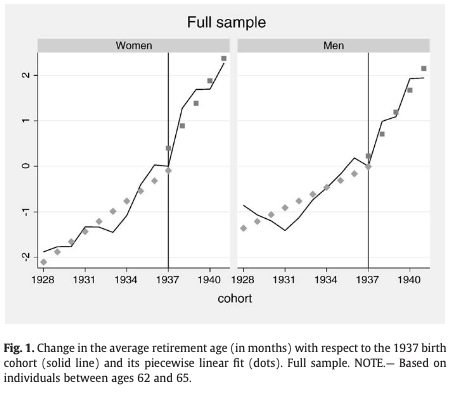
\includegraphics[width=8cm]{imgs/mastrobouni-fig1}
        \caption{Descriptivos}
        \label{fig:fig2}
      \end{figure}
  }
  \frame
  {
    \frametitle{Estrategia}
    \begin{itemize}
      \item Diff-in-diff
      \item Cohortes 1928-1937 (control)
      \item Cohortes 1938-1941 (tratamiento)
    \end{itemize}
  }
  \frame
  {
    \frametitle{Resultados}
      \begin{figure}[htp]
        \centering
        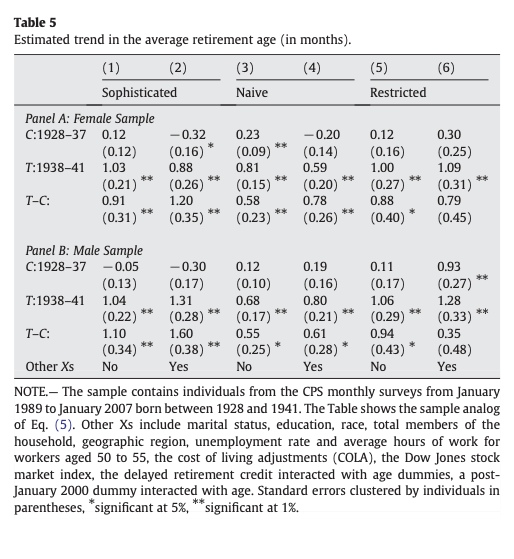
\includegraphics[width=8cm]{imgs/mastrobouni-tab5}
        \caption{Salida}
        \label{fig:fig2}
      \end{figure}
  }
  \frame
  {
    \frametitle{Discusión}
    \begin{itemize}
      \item El crecimiento de la edad promedio de retiro se acelera para los cohortes que enfrentan la nueva NRA.
      \item La edad efectiva de retiro aumenta 50\% del aumento de la NRA.
    \end{itemize}
  }
  \frame
  {
     \frametitle{Employment and substitution effects of raising the statutory retirement age in France}
     \begin{itemize}
       \item Francia, \textit{Régime Général}, cubre $\frac{2}{3}$ de la población.
       \item Suba gradual de la EMR de 60 a 62 en 2010.
       \item Hay un cambio en la ENR que afecta otras cohortes.
     \end{itemize}
  }
  \frame
  {
    \frametitle{Identificación}
      \begin{itemize}
        \item Evalúa el impacto de la suba de 60 a 61 sobre oferta laboral y sustitución por otros programas.
        \item La primera cohorte afectada es la nacida a finales de 1951, su ERA pasó a 60 años y 4 meses.
       \item La cohorte 1955 tiene una era de 62 años.
     \end{itemize}
  }
  \frame
  {
    \frametitle{Evidencia Descriptiva}
      \begin{figure}[htp]
        \centering
        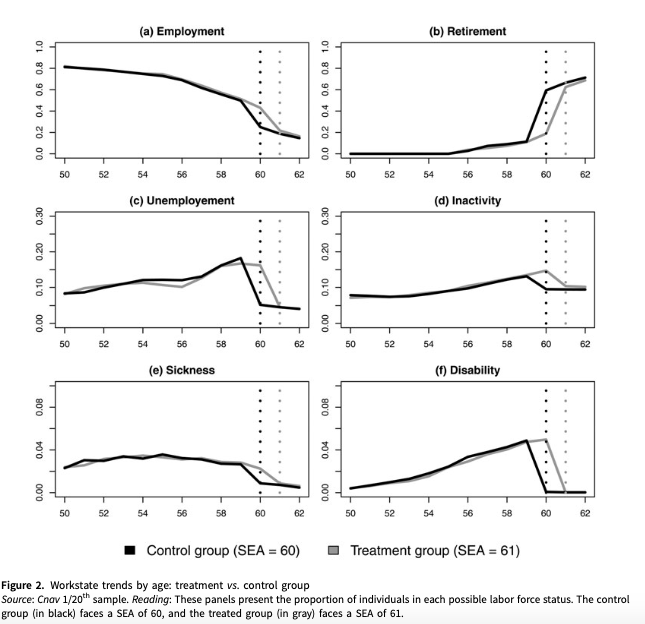
\includegraphics[width=8cm]{imgs/rabate-fig2}
        \caption{Descriptiva}
        \label{fig:fig2}
      \end{figure}
  }
  \frame
  {
    \frametitle{Evidencia Descriptiva}
        \begin{itemize}
        \item La cohorte de control tiene mayor probabilidad de retirarse (los trabajadores menores de la EMR pueden retirarse si tienen carreras de trabajo largas).
        \item Los miembros de la cohorte tratada tienen mayor probabilidad de estar trabajando.
        \item Los miembros de la cohorte tratada tienen mayor probabilidad de estar desempleados.
        \item Los miembros de la cohorte tratada tienen mayor probabilidad de estar inactivos, en seguro de enfermedad e invalidez.
     \end{itemize}
    
  }
  \frame
  {
    \frametitle{Varias especificaciones}
      \begin{figure}[htp]
        \centering
        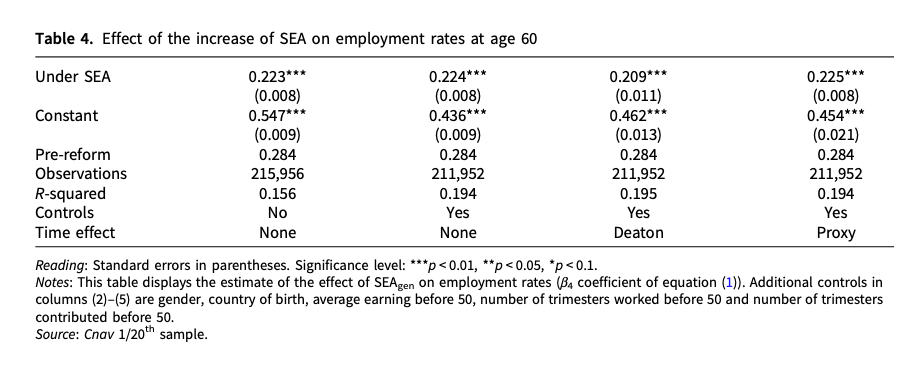
\includegraphics[width=12cm]{imgs/rabate-tab4}
        \label{fig:fig2}
      \end{figure}
  }
  \frame
  {
    \frametitle{Otros Estados}
      \begin{figure}[htp]
        \centering
        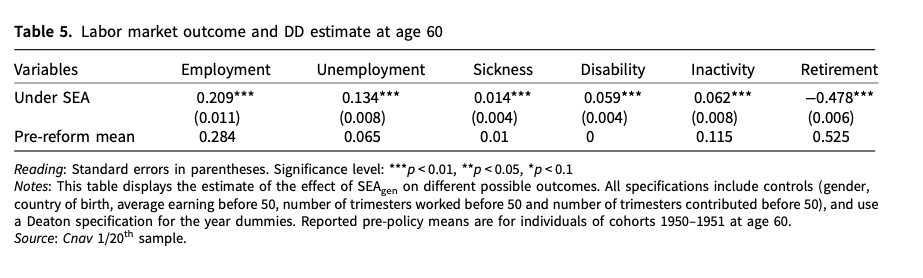
\includegraphics[width=12cm]{imgs/rabate-tab5}
        \label{fig:fig2}
      \end{figure}
  }
  \frame
  {
    \frametitle{Discusión}
    Las regresiones permiten controlar por X, Y, Z. Permiten establecer efectos causales de aumentar la EMR.
      \begin{itemize}
      \item La probabilidad de estar empleado sube aprox. 20\%.
      \item Efectos sustitución con otros programas altos (13.5 \% seguro de desempleo)
      \item Efectos menores pero significativos sobre invalidez, enfermedad e inactividad.
      \end{itemize}
  }
  \frame
  {
    \frametitle{Efectos Heterogéneos}
        \begin{figure}[htp]
        \centering
        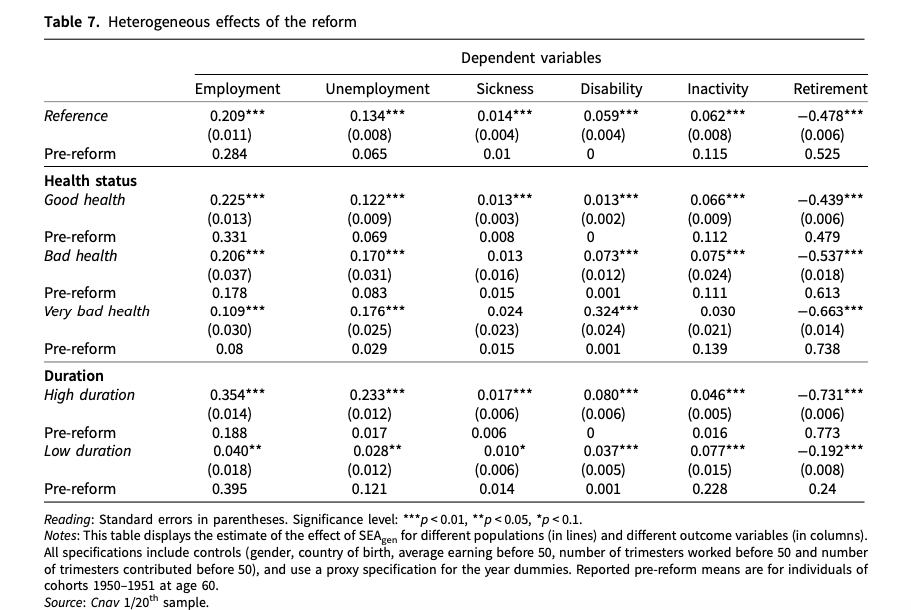
\includegraphics[width=12cm]{imgs/rabate-tab7}
        \label{fig:fig2}
      \end{figure}
    
  }
  
  \frame
  {
    \frametitle{Does Raising the Retirement Age Increase Employment of Older Workers?}
    \begin{itemize}
    \item Staubli y Zweimüller (2011 - IZA)
    \item Austria, aumento de la ERA en 2000 y 2004
    \item Cohortes afectadas:
    \item Compara las cohortes por debajo y por encima de la ERA.
    \end{itemize}
  }
  \frame
  {
    \frametitle{Evidencia Descriptiva}
      \begin{figure}[htp]
        \centering
        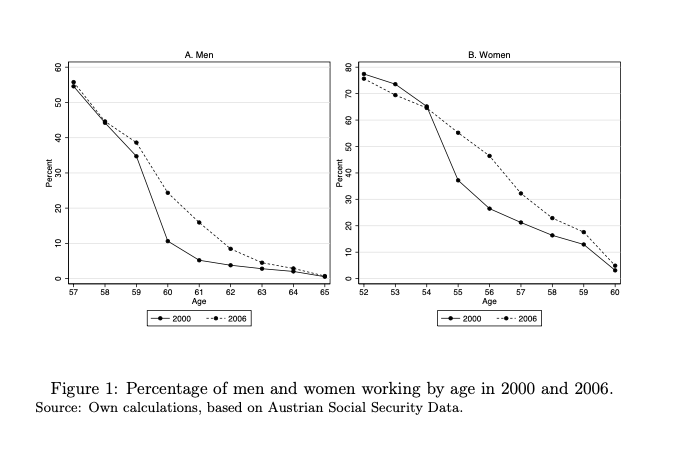
\includegraphics[width=10cm]{imgs/staubli-fig1}
        \caption{Evidencia}
        \label{fig:fig2}
      \end{figure}
  }
  \frame
  {
    \frametitle{Más evidencia descriptiva}
      \begin{figure}[htp]
        \centering
        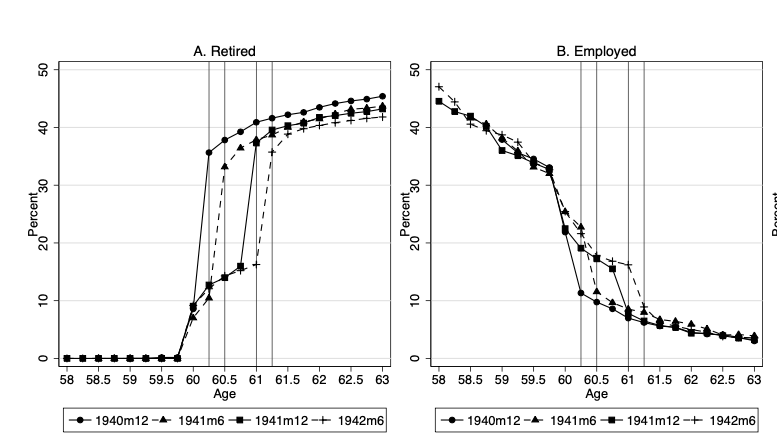
\includegraphics[width=10cm]{imgs/staubli-fig4}
        \caption{Salida 2}
        \label{fig:fig2}
      \end{figure}
  }
  \frame
  {
    \frametitle{Salida 1}
      \begin{figure}[htp]
        \centering
        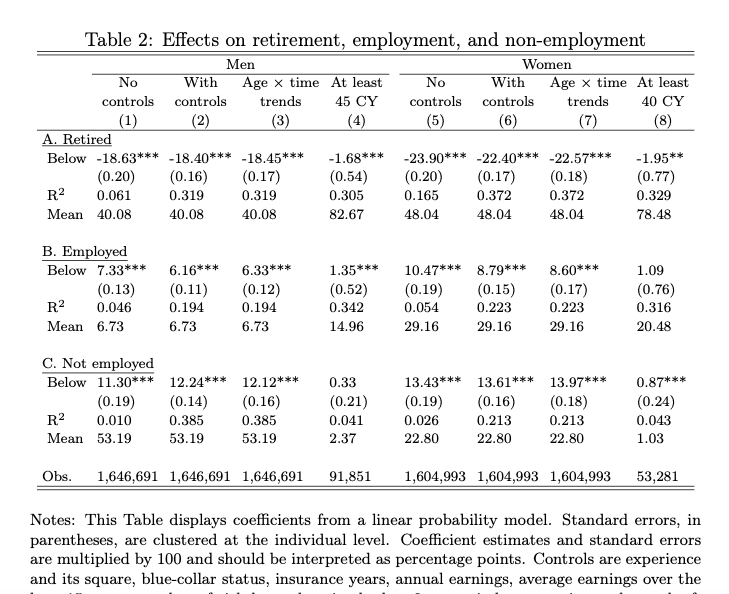
\includegraphics[width=10cm]{imgs/staubli-tab2}
        \caption{Salida 2}
        \label{fig:fig2}
      \end{figure}
  }
  \frame
  {
    \frametitle{Salida 1}
      \begin{figure}[htp]
        \centering
        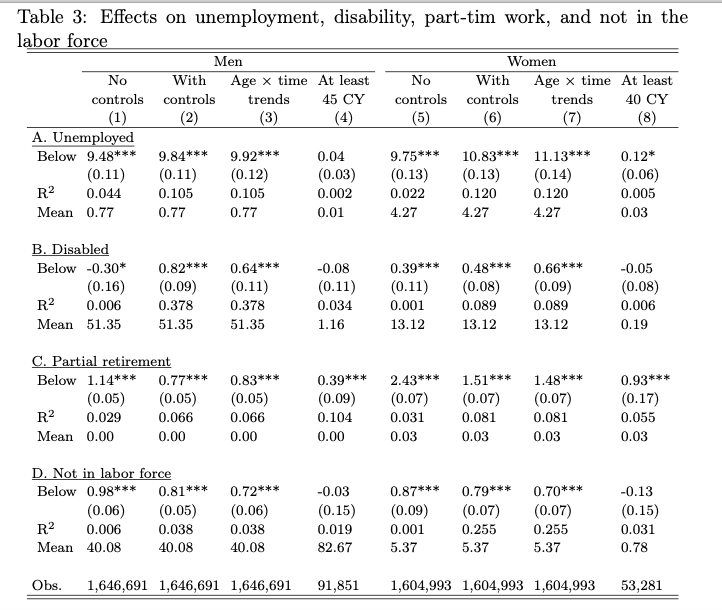
\includegraphics[width=10cm]{imgs/staubli-tab3}
        \caption{Salida 2}
        \label{fig:fig2}
      \end{figure}
  }
  \frame
  {
    \frametitle{Financial incentives to postpone retirement and further effects on employment}
    \begin{itemize}
    \item Hanel, 2010
    \item Alemania
    \item Reducción de prestaciones por retiro temprano.
    \end{itemize}
  }
  \frame
  {
    \frametitle{Evidencia Descriptiva}
      \begin{figure}[htp]
        \centering
        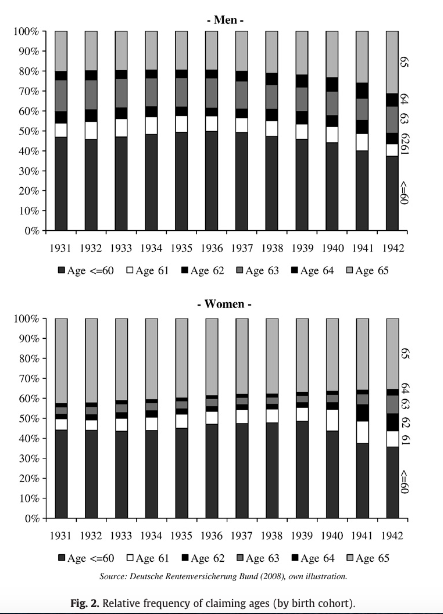
\includegraphics[width=10cm]{imgs/hanel10-fig2}
        \caption{Salida 2}
        \label{fig:fig2}
      \end{figure}
  }
  \frame
  {
    \frametitle{Evidencia Descriptiva1}
      \begin{figure}[htp]
        \centering
        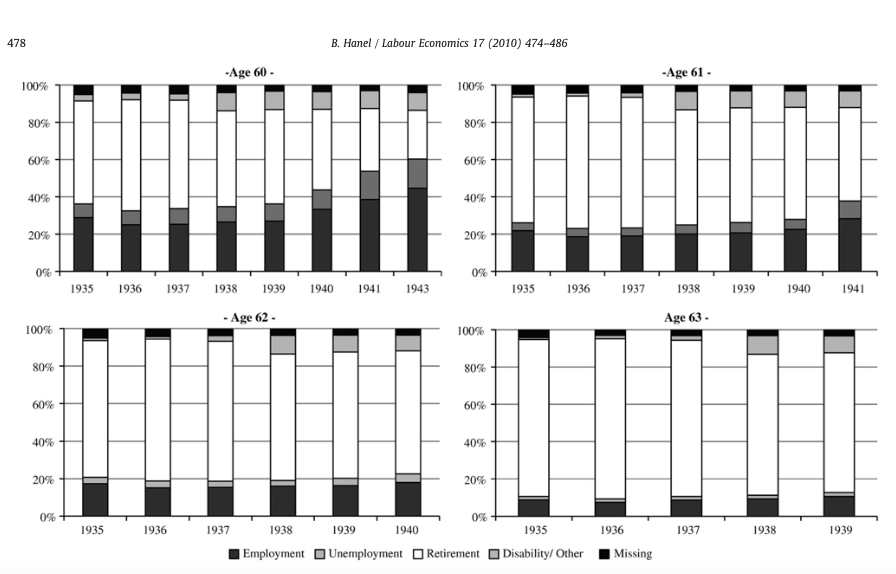
\includegraphics[width=10cm]{imgs/hanel10-fig3}
        \caption{Salida 2}
        \label{fig:fig2}
      \end{figure}
  }
  \frame
  {
    \frametitle{Salida}
      \begin{figure}[htp]
        \centering
        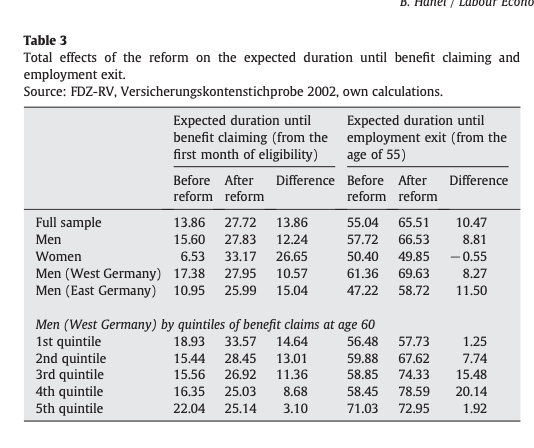
\includegraphics[width=10cm]{imgs/hanel10-tab3}
        \caption{Salida 2}
        \label{fig:fig2}
      \end{figure}
  }
  \frame
   {
     \frametitle{Labour Supply effects of early retirement provision}
     \begin{itemize}
     \item Noruega
     \item Baja de la ERA de 64 a 62. 
     \end{itemize}
   }

       \frame
           {
             \frametitle{Política: AFP}
             \begin{itemize}
             \item Es un programa de retiro temprano voluntario al que acceden los trabajadores del sector público y la mitad de los trabajadores privados.
             \item Al principio la edad mínima era 66, se redujo gradualmente a 62 entre 1990 y 1998.
             \item La edad de retiro normal era 67, y antes de 1989 no había opciones de retiro temprano.
             \item Los programas de desempleo e invalidez funcionaban como vías de salida del mercado laboral.

             \end{itemize}
           }
      \frame
           {
             \frametitle{AFP: Beneficios}
             \begin{itemize}
             \item No hay ajustes actuariales
             \end{itemize}
           }
           
    \frame
    {
    \frametitle{Evidencia descriptiva}
    
    \begin{figure}[htp]
      \centering
      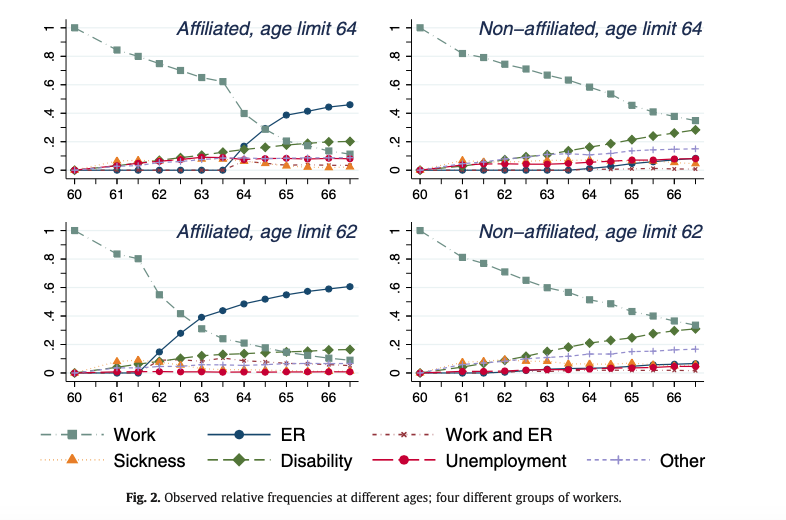
\includegraphics[width=8cm]{imgs/vestad-fig2}
      \caption{Descriptivos}
      \label{fig:fig2}
    \end{figure}
    }
           \frame {
             \frametitle{Estrategia empírica}
             \begin{itemize}
             \item Diff-in-diff usando el grupo de trabajadores con ERA 62 con el de ERA 64.
             \item $Y_{ict}$ es el estado relevante (trabajando, en seguro de desmpleo o en seguro de invalidez).
             \end{itemize}
             
             \begin{align*}
               y_{ict} &= \alpha + \beta_{1}X_{i} + \beta_{2} \tau_{t} + \beta_{3} \delta_{c} + \beta_{4}D_{i} \\
               &+ \beta_{5} (\delta_{c} \times \tau_{t}) + \beta_{6} ( D_{i} \times \tau_{t}) + \beta_{7} (D_{i} \times \tau_{t}) \\
               &+ \beta_{8} (\delta_{c} \times \tau_{t} \times D_{i})
             \end{align*}

           }

    \frame
    {
    \frametitle{Salida}
    
    \begin{figure}[htp]
      \centering
      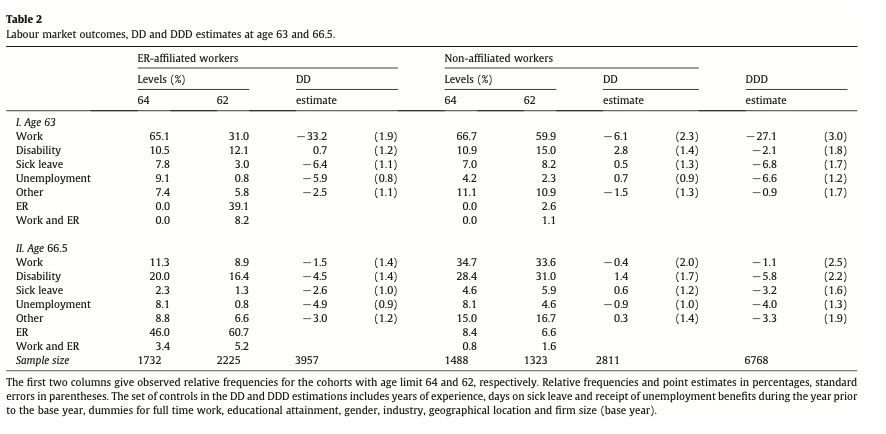
\includegraphics[width=14cm]{imgs/vestad-tbl2}
      \caption{Descriptivos}
      \label{fig:fig2}
    \end{figure}
    }
   \frame {
     \frametitle{Resultados y discusión}
        \begin{itemize}
        \item Se estiman los efectos en la oferta de trabajo de cambios en la edad mínima de retiro, caracterizando el impacto sobre distintos caminos hacia el retiro y la sustitución entre programas.
       \item La mitad de los jubilados por el programa de retiro temprano estarían trabajando a los 66.5 años sin el programa.
       \item 70\% estarían trabajando a los 63 si la edad fuera 64.
       \item El principal programa sustituto es la pensión por invalidez.
       \end{itemize}


}
\frame
    {
      \frametitle{The Impact of Pension Eligibility Age on Retirement }
      \begin{itemize}
      \item Estudian  que el aumento de la edad mínima de retiro para las mujeres en Australia en 1993.
      \item Encuentran reduce 8\% la probabilidad de retirarse.
      \item Encuentran que hay sustitución de programas
      \end{itemize}
    }
    \frame
        {
          \frametitle{Preguntas}

          \begin{itemize}
          \item Medir el impacto del cambio en la edad mínima de retiro en la oferta laboral
          \item Medir la sustitución por otros programas
          \end{itemize}

          }
    \frame
        {
          \frametitle{Canales}

          El cambio en la edad de retiro afecta la decisión de retiro por dos canales:
          \begin{itemize}
          \item Reduce la riqueza del individuo, induciéndolo a consumir menos ocio.
          \item Aumenta las contribuciones, y por ende los beneficios (en algunos casos).
          \end{itemize}

          Ambos efectos tienen el mismo signo cuando aumenta la edad de retiro, por lo que puede ser difícil separarlos. En el caso de Australia, el segundo efecto no opera, por lo que es un experimento para estudiar el primer efecto aislado.

        }
        \frame
            {
              \frametitle{Antecedentes}
              \begin{itemize}
              \item La mayor parte de los trabajos anteriores usan variación cross-section
                ~\cite{coile}.

              \item Se encuentran efectos fuertes de \textit{accrual effects}.
              \item Usan simulaciones y predicciones \textit{out of sample}.
              \item Problemas para tomar en cuenta comportamientos asociados a normas de comportamiento.
              \item Problemas de identificación: cómo separar el efecto
                de los parámetros del sistema y de las tendencias de retiro.
              \end{itemize}

            }
            \frame
                {
                  \frametitle{Variación exógena}

                  \begin{itemize}
                  \item La solución es encontrar una variación exógena para identificar los efectos

                  \item El pionero es \cite{krueger}, también es importante \cite{mastrobouni}.
                  \item Trabajos similares a este son Hanel (para Suiza).
                  \item Otro grupo de trabajos que analizan los impactos de cambios en los parámetros de la Seguridad Social en la sustitución de programas.

                  \end{itemize}
                  }
                \frame
                    {

                      \frametitle{Este trabajo}

                      \begin{itemize}
                      \item Busca aislar el efecto riqueza.
                      \item Encuentran que el efecto de subir la edad mínima de retiro aumentó puntos porcentuales la participación de las mujeres en el mercado laboral.
                      \item Encuentran efectos significativos en el uso de otros programas, especialmente invalidez.
                      \end{itemize}
                      }

\end{document}
